% ============================================================
% Recueil COMIMa — Techniques de résolution de problèmes
% Chapitre 0 — Exemples et contre-exemples
%
% Compilation (paquet .tex exporté) : latexmk -pdf cours.tex
% Les énoncés et solutions des exercices sont inclus depuis
% <id>/enonce.tex et <id>/solution.tex (content/exercices/ sur le dépôt).
% ============================================================
\documentclass[11pt]{article}
\input{preamble.tex}
\input{preamble-cours.tex}

% Solutions en fin de chapitre : \solutionsfalse pour les masquer.
\solutionstrue

\begin{document}
% Pagination du recueil : le chapitre 0 commence page 5.
\setcounter{page}{5}

\chapitre{0}{Exemples et contre-exemples}

En mathématiques, on commence souvent par calculer quelques cas, dessiner
quelques figures, et l'on voit apparaître une régularité. C'est une étape
indispensable : elle permet de \emph{deviner}. Mais deviner n'est pas
démontrer. Ce chapitre montre, sur des exemples simples, pourquoi des
vérifications, même très nombreuses, ne prouvent pas un énoncé général, et
pourquoi un seul contre-exemple suffit à le réfuter.

% ------------------------------------------------------------
\section{Exemple introductif : des points sur un cercle}

On place $n$ points sur un cercle et on trace toutes les cordes qui les
relient deux à deux, en choisissant les points de sorte que trois cordes ne
soient jamais concourantes en un point intérieur. Combien de régions
obtient-on à l'intérieur du disque ?

\begin{center}
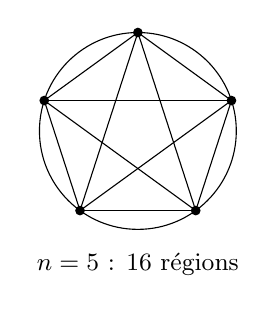
\begin{tikzpicture}[scale=1.25]
  \draw (0,0) circle (1);
  \foreach \a in {90,162,234,306,18} \fill (\a:1) circle (1.4pt);
  \foreach \a/\b in {90/162,90/234,90/306,90/18,162/234,162/306,162/18,234/306,234/18,306/18}
    \draw (\a:1) -- (\b:1);
  \node at (0,-1.35) {\small $n = 5$ : $16$ régions};
\end{tikzpicture}
\end{center}

\needspace{6\baselineskip}
En comptant sur des figures, on obtient :
\begin{center}
\begin{tabular}{c|ccccc}
  nombre de points $n$ & $1$ & $2$ & $3$ & $4$ & $5$ \\ \hline
  nombre de régions    & $1$ & $2$ & $4$ & $8$ & $16$
\end{tabular}
\end{center}
Le nombre de régions semble doubler à chaque point ajouté : on est tenté
d'affirmer qu'il vaut $2^{n-1}$. Pourtant, avec $n = 6$ points, une figure
soignée ne donne que $31$ régions, et non $32$.

\medskip
Cinq vérifications concordantes ne prouvaient donc rien. On peut démontrer,
avec des outils de dénombrement, que le nombre de régions vaut en réalité
\[
1 + \binom{n}{2} + \binom{n}{4},
\]
ce qui donne bien $1, 2, 4, 8, 16$ pour $n = 1, \ldots, 5$, puis $31$ pour
$n = 6$ et $57$ pour $n = 7$.

% ------------------------------------------------------------
\section{Conjectures, preuves et contre-exemples}

\begin{definition}
Une \emph{conjecture} est un énoncé que l'on pense vrai, souvent au vu
d'exemples, mais qui n'est pas encore démontré.
\end{definition}

Beaucoup d'énoncés sont \emph{universels} : ils affirment qu'une propriété
$\mathcal{P}(n)$ est vraie \emph{pour tout} élément $n$ d'un ensemble $E$,
ce que l'on note $\forall n \in E,\ \mathcal{P}(n)$.

\begin{definition}
Un \emph{contre-exemple} à l'énoncé $\forall n \in E,\ \mathcal{P}(n)$ est
un élément $n_0 \in E$ pour lequel $\mathcal{P}(n_0)$ est fausse.
\end{definition}

La négation de \og pour tout $n$, $\mathcal{P}(n)$ \fg{} est \og il existe
$n$ tel que $\mathcal{P}(n)$ soit fausse \fg :
\[
\text{non}\bigl(\forall n \in E,\ \mathcal{P}(n)\bigr)
\iff \exists n \in E,\ \text{non}\,\mathcal{P}(n).
\]
On en tire les deux principes de ce chapitre.
\needspace{9\baselineskip}

\begin{proposition}\label{prop:principes}
Soit $E$ un ensemble et $\mathcal{P}(n)$ une propriété.
\begin{enumerate}
  \item Pour \emph{réfuter} l'énoncé $\forall n \in E,\ \mathcal{P}(n)$, il
  suffit d'exhiber \emph{un seul} contre-exemple.
  \item Si $E$ est \emph{infini}, des exemples ne suffisent jamais à
  \emph{démontrer} cet énoncé, aussi nombreux soient-ils : il faut un
  raisonnement valable pour tout $n \in E$.
\end{enumerate}
\end{proposition}

\begin{remarque}
Si $E$ est \emph{fini}, vérifier tous les cas un par un est une
démonstration (une \og vérification exhaustive \fg). À l'inverse, pour
démontrer un énoncé \emph{existentiel}, \og il existe $n \in E$ tel que
$\mathcal{P}(n)$ \fg, un seul exemple suffit : par exemple, $3$ et $5$ sont
premiers, donc il existe un nombre premier $p$ tel que $p + 2$ soit premier.
\end{remarque}

\begin{exemple}
On calcule les sommes des premiers nombres impairs :
\[
1 = 1, \quad 1 + 3 = 4, \quad 1 + 3 + 5 = 9, \quad 1 + 3 + 5 + 7 = 16 .
\]
On \emph{conjecture} que, pour tout $n \geqslant 1$,
$1 + 3 + 5 + \cdots + (2n - 1) = n^2$. Cette fois, la conjecture est vraie,
mais il faut la démontrer. Pour tout $k \geqslant 1$,
$k^2 - (k-1)^2 = 2k - 1$. En additionnant ces égalités pour
$k = 1, \ldots, n$, les termes intermédiaires se simplifient :
\[
\sum_{k=1}^{n} (2k - 1) = \sum_{k=1}^{n} \bigl(k^2 - (k-1)^2\bigr) = n^2 - 0^2 = n^2 .
\]
\end{exemple}

% ------------------------------------------------------------
\section{Méthode : chercher, conjecturer, puis trancher}

Face à un énoncé général, on peut procéder ainsi.
\begin{enumerate}
  \item \emph{Explorer.} Calculer ou dessiner plusieurs cas, de façon
  organisée (un tableau de valeurs, des figures variées).
  \item \emph{Conjecturer.} Formuler précisément l'énoncé que suggèrent les
  exemples.
  \item \emph{Chercher un contre-exemple.} Les contre-exemples se cachent
  souvent :
  \begin{itemize}
    \item dans les petites valeurs et les cas limites ($n = 0$, $n = 1$) ;
    \item dans les grandes valeurs, quand la propriété résiste longtemps ;
    \item dans les figures que l'on ne dessine pas spontanément (polygone
    non convexe, triangle très aplati) ;
    \item dans une hypothèse implicite que l'énoncé ne contient pas.
  \end{itemize}
  \item \emph{Trancher.} Soit on exhibe un contre-exemple, et l'énoncé est
  faux ; soit on trouve un raisonnement général, et l'énoncé devient un
  théorème.
\end{enumerate}

% ------------------------------------------------------------
\section{À retenir}

\begin{retenir}
\begin{itemize}
  \item Des exemples permettent de deviner, jamais de démontrer un énoncé
  portant sur une infinité de cas (sur un ensemble fini, vérifier tous les cas
  est une démonstration).
  \item Un contre-exemple à $\forall n \in E,\ \mathcal{P}(n)$ est un $n_0 \in E$
  tel que $\mathcal{P}(n_0)$ soit fausse ; un seul suffit à réfuter un énoncé
  universel.
  \item Pour un énoncé \emph{existentiel}, un seul exemple suffit à le démontrer.
  \item La négation de \og pour tout $n$, $\mathcal{P}(n)$ \fg{} est
  \og il existe $n$ tel que $\mathcal{P}(n)$ soit fausse \fg.
  \item Une conjecture peut être vraie : il faut alors la démontrer.
  \item Penser aux cas limites et aux figures inhabituelles.
\end{itemize}
\end{retenir}

% ------------------------------------------------------------
\section{Exercices}

\exochap{recueil-0-01-factorielle-puissances}{Factorielle et puissances}
\exochap{recueil-0-02-inegalite-factorielle}{Une inégalité avec des factorielles}
\exochap{recueil-0-03-diagonales-polygone}{Les diagonales d'un polygone}
\exochap{recueil-0-04-valeurs-de-n}{Pour quelles valeurs de $n$ ?}
\exochap{recueil-0-05-polynome-premiers}{Un polynôme et des nombres premiers}
\exochap{recueil-0-06-somme-cubes}{La somme des cubes}
\exochap{recueil-0-07-suite-factorielle}{La suite $n! + 1$}
\exochap{recueil-0-08-angles-pentagone}{Les angles d'un pentagone}
\exochap{recueil-0-09-medianes-triangle}{Les médianes d'un triangle}
\exochap{recueil-0-10-vrai-ou-faux}{Vrai ou faux ?}
\exochap{recueil-0-11-votre-enonce}{Proposez votre énoncé}
\exochap{recueil-0-12-conjecture-collatz}{La conjecture de Collatz}

% ------------------------------------------------------------
\ifsolutions
\clearpage
\section{Solutions}

\solutionde{recueil-0-01-factorielle-puissances}{Factorielle et puissances}{ex}
\solutionde{recueil-0-02-inegalite-factorielle}{Une inégalité avec des factorielles}{ex}
\solutionde{recueil-0-03-diagonales-polygone}{Les diagonales d'un polygone}{ex}
\solutionde{recueil-0-04-valeurs-de-n}{Pour quelles valeurs de $n$ ?}{ex}
\solutionde{recueil-0-05-polynome-premiers}{Un polynôme et des nombres premiers}{ex}
\solutionde{recueil-0-06-somme-cubes}{La somme des cubes}{ex}
\solutionde{recueil-0-07-suite-factorielle}{La suite $n! + 1$}{ex}
\solutionde{recueil-0-08-angles-pentagone}{Les angles d'un pentagone}{ex}
\solutionde{recueil-0-09-medianes-triangle}{Les médianes d'un triangle}{ex}
\solutionde{recueil-0-10-vrai-ou-faux}{Vrai ou faux ?}{ex}
\solutionde{recueil-0-11-votre-enonce}{Proposez votre énoncé}{ex}
\solutionde{recueil-0-12-conjecture-collatz}{La conjecture de Collatz}{ex}
\fi

\end{document}
